\documentclass[UTF8,aspectratio=169,11pt]{ctexbeamer}

\usetheme{Madrid}
\usecolortheme{default}
\usepackage{amsmath}
\usepackage{booktabs}
\usepackage{graphicx}
\usepackage{hyperref}
\usepackage{xcolor}

\graphicspath{{../assets/}}
\setbeamertemplate{navigation symbols}{}
\setbeamertemplate{caption}[numbered]
\definecolor{Ink}{HTML}{1F2937}
\definecolor{Accent}{HTML}{0F766E}
\setbeamercolor{title}{fg=Ink}
\setbeamercolor{frametitle}{fg=Ink}
\setbeamercolor{structure}{fg=Accent}

\title[Experiments]{Experiments\\高维两样本 MSWD 检验复现实验}
\author{MSWD Bootstrapping Reproduction}
\date{\today}

\begin{document}
\section{Experiments}

\begin{frame}[plain]
  \titlepage
\end{frame}

\begin{frame}{论文方法如何连接三个实验}
\begin{itemize}
  \item 目标：检验 \(H_0:P=Q\) 对 \(H_1:P\neq Q\)，允许 \(p\) 很大。
  \item 核心统计量：在稀疏方向上最大化一维 Wasserstein 距离。
  \[
  T_n=\left(\frac{n_1n_2}{n_1+n_2}\right)^{1/2}
  \sup_{v\in V_{0,s}} W_1(v^\top X,v^\top Y).
  \]
  \item 判定：观测 \(T_n\) 超过 bootstrap 零分布的 \(1-\alpha\) 分位数则拒绝。
  \item SCI：同一套 bootstrap 机制还能定位显著边际变量和 GO term 子集。
\end{itemize}
\end{frame}

\begin{frame}{三个实验的角色}
\begin{tabular}{p{0.22\linewidth}p{0.34\linewidth}p{0.34\linewidth}}
\toprule
实验 & 问题 & 输出 \\
\midrule
Model A 方法对比 & MSWD 在论文核心仿真场景下是否有 power 优势 & 50 次运行的经验拒绝率曲线 \\
MSWD 单独 bootstrap & 一次样本下统计量如何与零分布比较 & 观测 \(T_n\)、bootstrap 阈值、p-value \\
GBM 真实数据 & LGG 与 GBM 甲基化分布是否不同，差异在哪里 & 全局检验、138 个边际基因、7 个 GO term \\
\bottomrule
\end{tabular}
\end{frame}

\begin{frame}{实验一配置：Model A 前 50 次 Monte Carlo}
\begin{itemize}
  \item 模型：\(X\sim N(0_p,\Sigma)\)，\(Y\sim N(\mu,\Sigma)\)。
  \item 协方差：\(\Sigma_{ij}=0.5^{|i-j|}\)。
  \item 均值衰减：\(\mu_j=0.8\beta j^{-3}\)。
  \item 参数：\(n_1=n_2=250\)，\(p=500\)，\(\alpha=0.05\)。
  \item 信号：\(\beta=0,0.2,0.4,0.6,0.8,1.0\)。
  \item 每个 \(\beta\) 写作 50 次完整实验；Proposed 方法 bootstrap \(B=300\)。
  \item 对比：MMD-G、ED$_2$、BG、PW；MMD-L 不能从日志恢复。
\end{itemize}
\end{frame}

\begin{frame}{实验一结果：Proposed power 上升最快}
\begin{center}
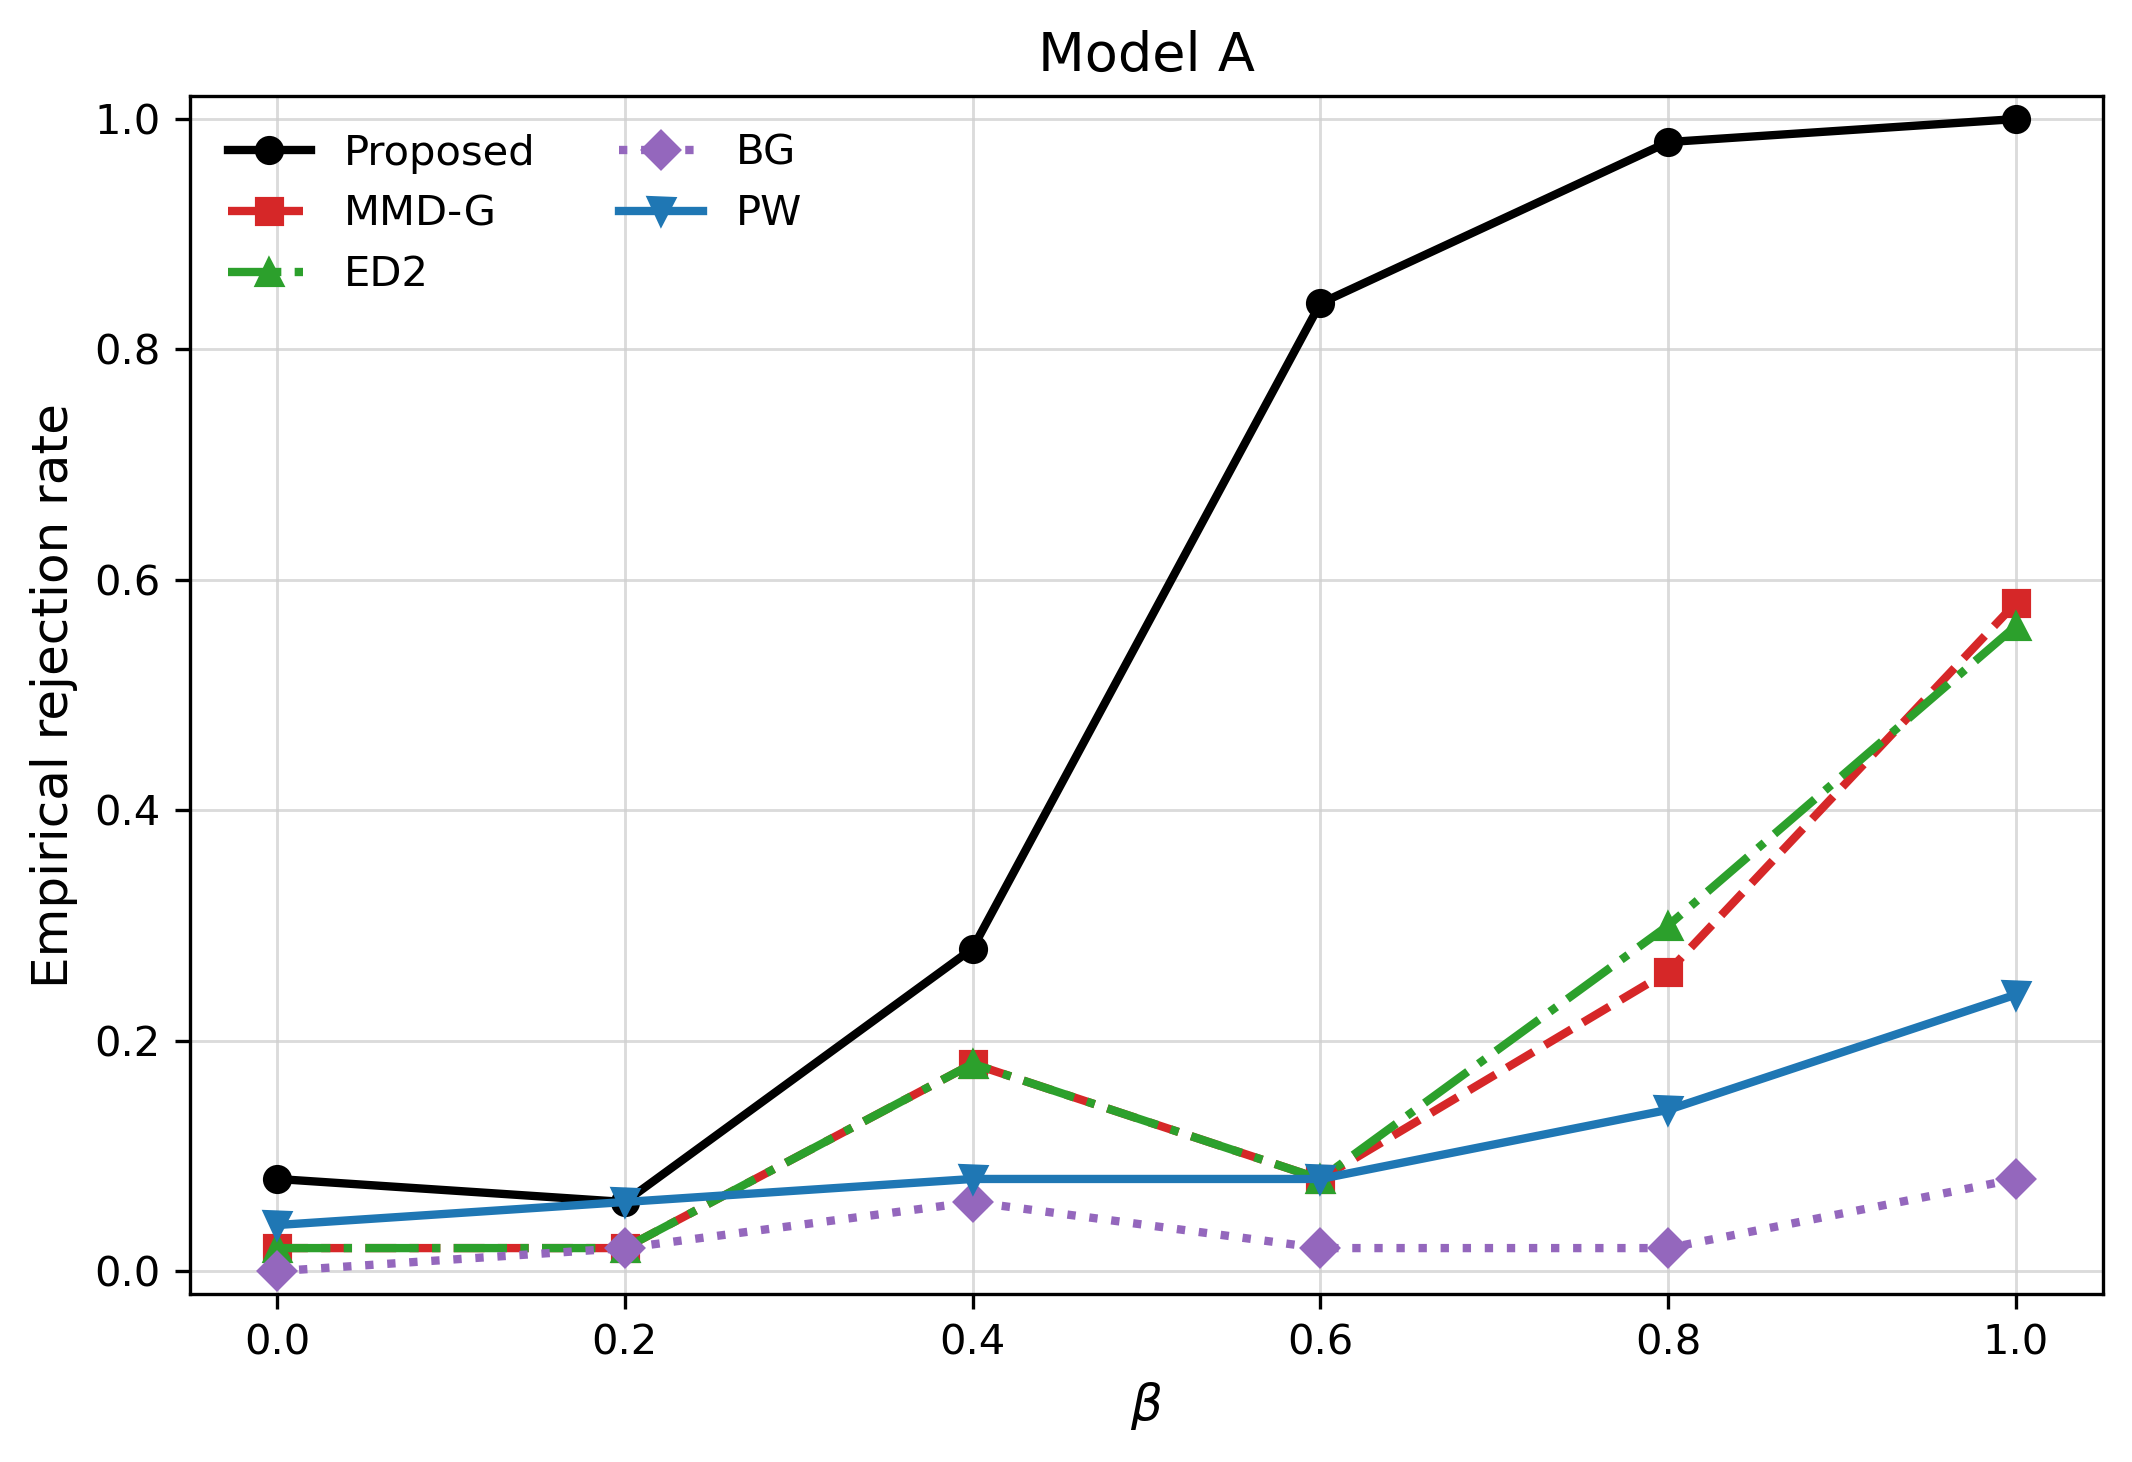
\includegraphics[width=0.82\linewidth,height=0.74\textheight,keepaspectratio]{fig1.png}
\end{center}
\end{frame}

\begin{frame}{实验一解读}
\small
\begin{tabular}{cccccc}
\toprule
\(\beta\) & Proposed & MMD-G & ED$_2$ & BG & PW \\
\midrule
0.0 & 0.08 & 0.02 & 0.02 & 0.00 & 0.04 \\
0.4 & 0.28 & 0.18 & 0.18 & 0.06 & 0.08 \\
0.6 & 0.84 & 0.08 & 0.08 & 0.02 & 0.08 \\
0.8 & 0.98 & 0.26 & 0.30 & 0.02 & 0.14 \\
1.0 & 1.00 & 0.58 & 0.56 & 0.08 & 0.24 \\
\bottomrule
\end{tabular}

\vspace{0.25cm}
\begin{itemize}
  \item \(\beta=0\) 下 size 约 0.08，50 次实验下可视为 Monte Carlo 波动。
  \item \(\beta=0.6\) 后 Proposed 明显拉开差距，符合论文对稀疏衰减信号的判断。
\end{itemize}
\end{frame}

\begin{frame}{实验二配置：单样本 MSWD bootstrap}
\begin{itemize}
  \item 每个 \(\beta\) 只生成一组 Model A 数据。
  \item 对这一组数据做 \(B=500\) 次 bootstrap。
  \item 目的不是估计 power，而是展示拒绝机制。
  \item 拒绝规则：observed \(T_n\) 大于 bootstrap 95\% 阈值。
  \item 参数：\(n_1=n_2=250\)，\(p=500\)，\(\alpha=0.05\)。
\end{itemize}
\end{frame}

\begin{frame}{实验二结果：强信号下观测统计量超过阈值}
\begin{center}
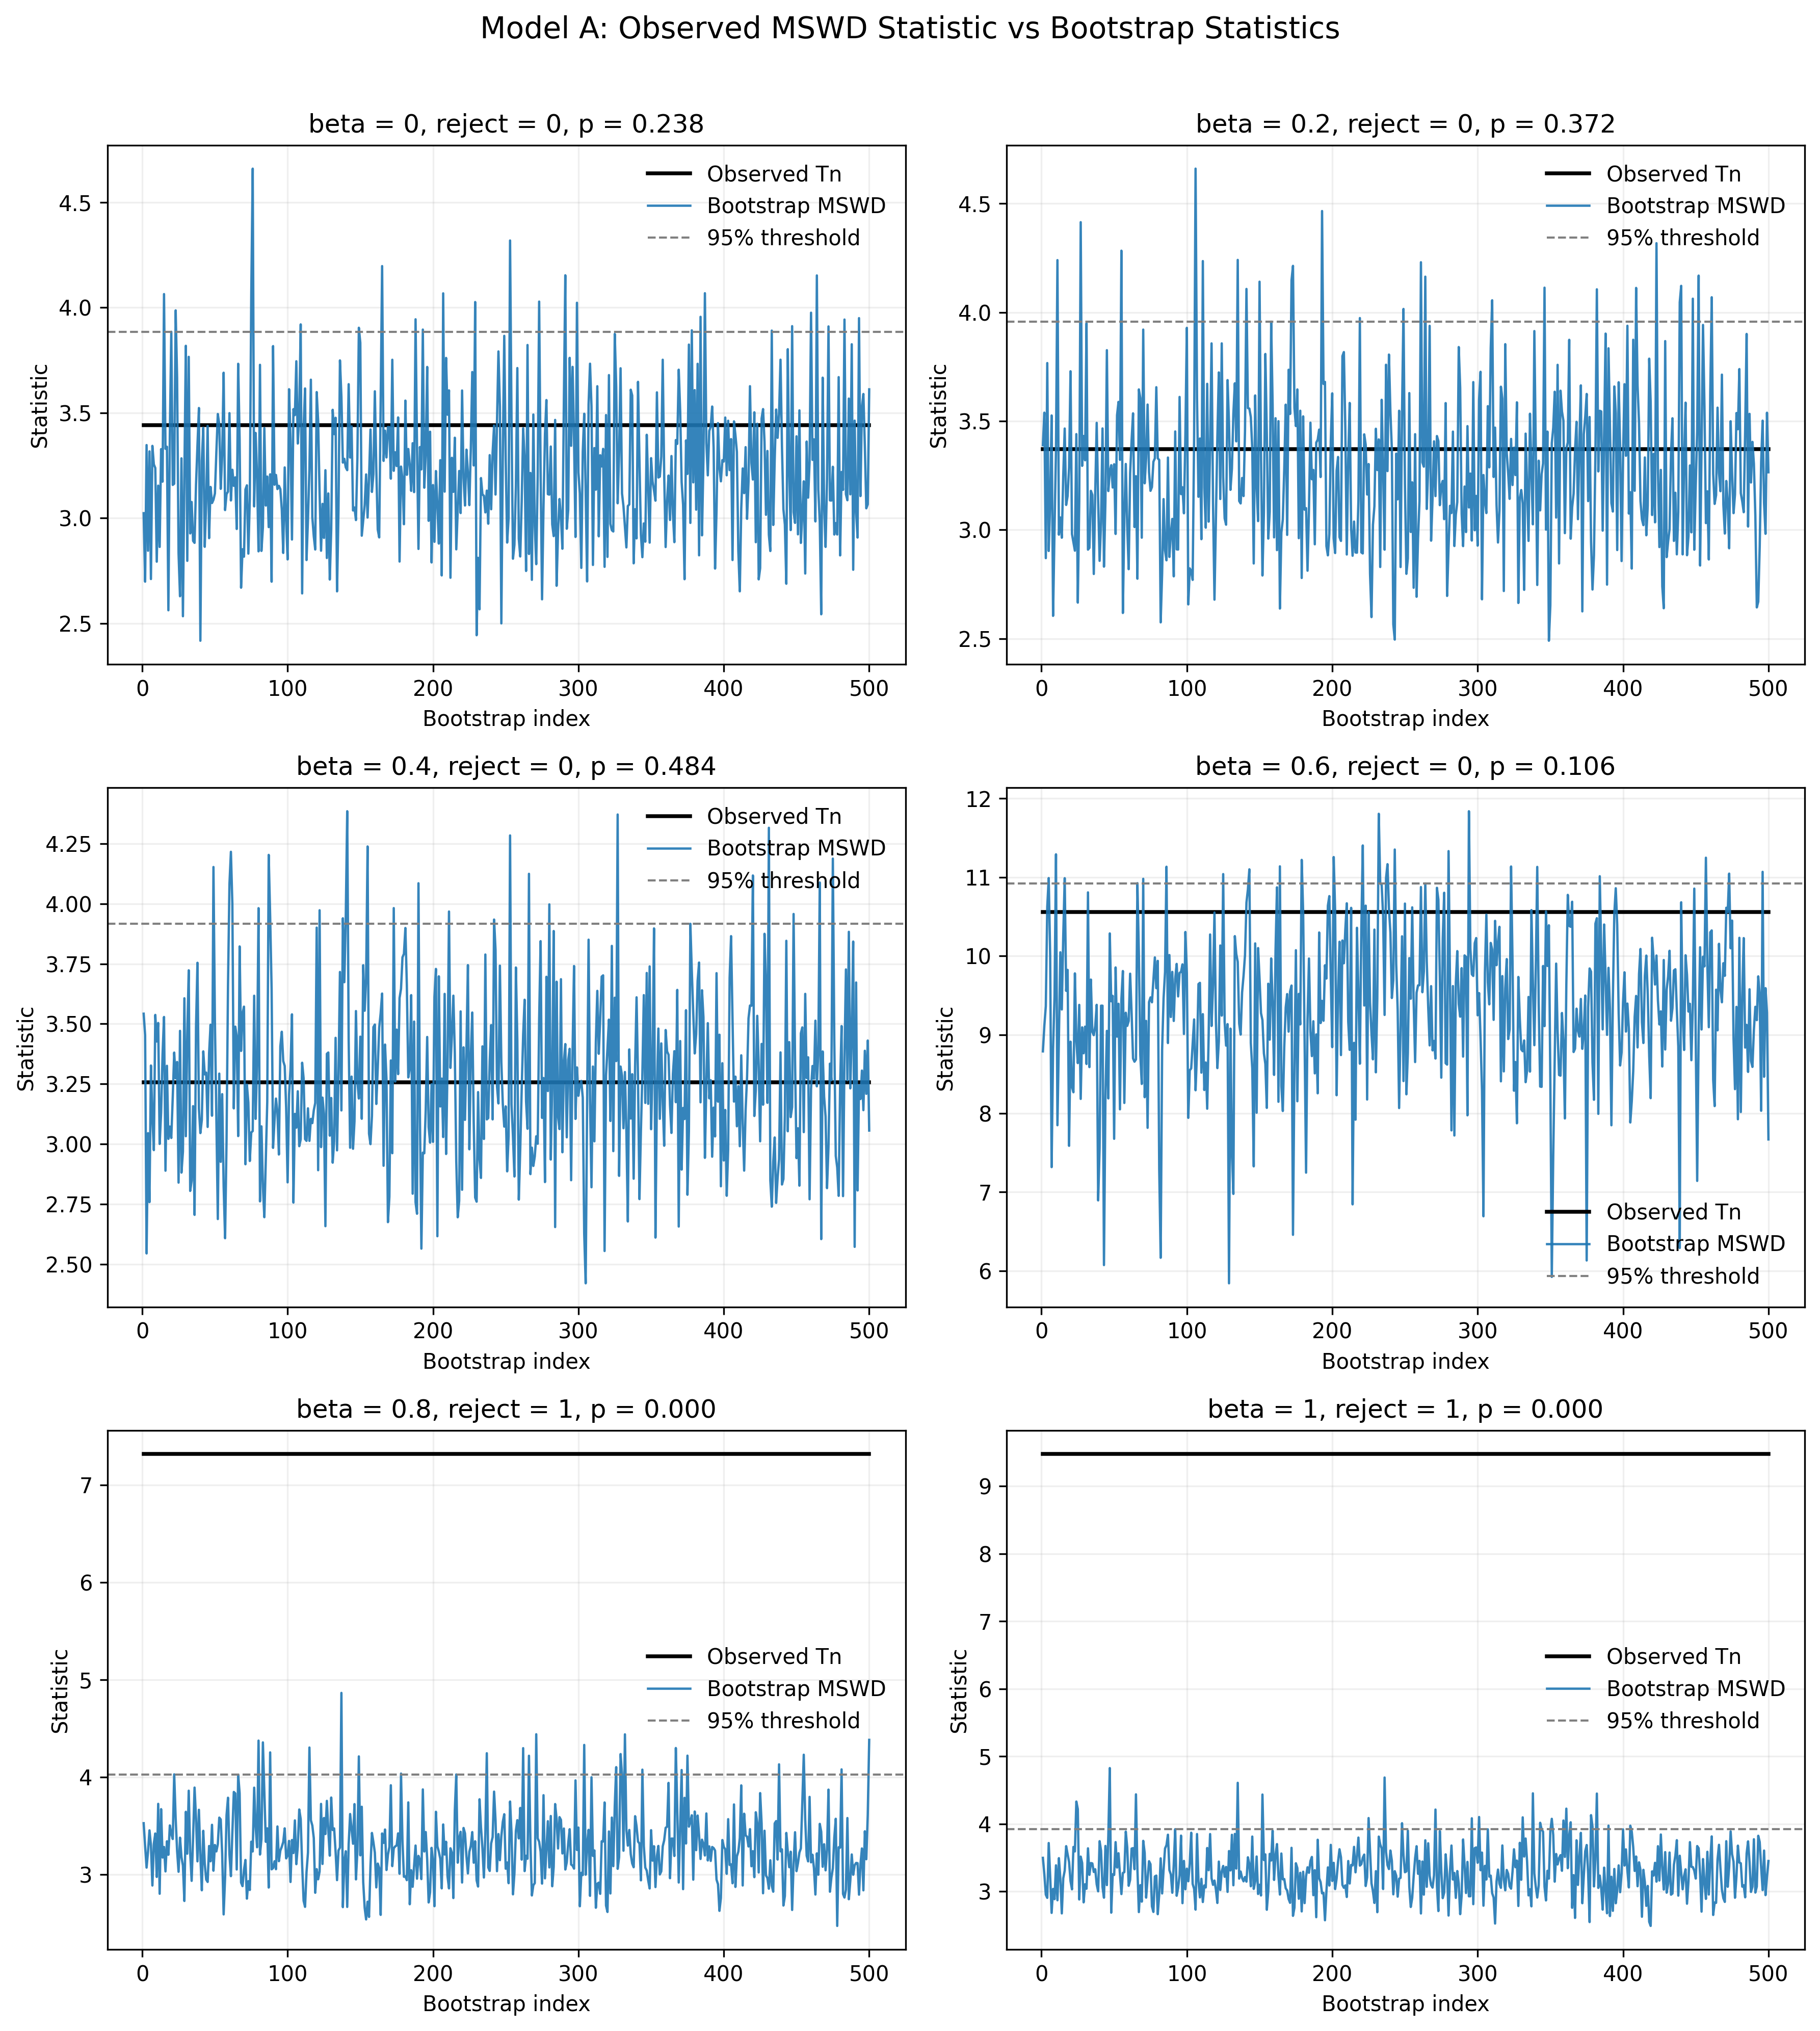
\includegraphics[width=0.84\linewidth,height=0.74\textheight,keepaspectratio]{fig2.png}
\end{center}
\end{frame}

\begin{frame}{实验二解读}
\small
\begin{tabular}{ccccc}
\toprule
\(\beta\) & observed \(T_n\) & threshold & p-value & reject \\
\midrule
0.0 & 3.442 & 3.885 & 0.238 & 否 \\
0.2 & 3.372 & 3.958 & 0.372 & 否 \\
0.4 & 3.256 & 3.918 & 0.484 & 否 \\
0.6 & 10.557 & 10.920 & 0.106 & 否 \\
0.8 & 7.319 & 4.025 & 0.000 & 是 \\
1.0 & 9.479 & 3.921 & 0.000 & 是 \\
\bottomrule
\end{tabular}

\vspace{0.25cm}
\begin{itemize}
  \item \(\beta=0.6\) 是边界附近未拒绝；这不等同于 power 低。
  \item 500 次 bootstrap 下 p-value 为 0，应写作 \(p<0.002\)。
\end{itemize}
\end{frame}

\begin{frame}{实验三配置：LGG/GBM DNA 甲基化}
\begin{itemize}
  \item 数据：TCGA LGG 与 GBM DNA methylation。
  \item 样本：\(n_1=511\) 个 LGG，\(n_2=150\) 个 GBM。
  \item 变量：\(p=207\) 个 glioma prognosis 相关基因。
  \item 方法：L0 sparse MSWD + bootstrap，\(B=500\)，\(\alpha=0.05\)。
  \item 目标：检验两组 207 维甲基化分布是否相同，并定位差异。
\end{itemize}
\end{frame}

\begin{frame}{实验三全局结果：LGG 与 GBM 显著不同}
\begin{tabular}{lc}
\toprule
指标 & 数值 \\
\midrule
检验统计量 & 42.9236 \\
bootstrap 临界值 & 1.8479 \\
经验 p-value & \(p<0.002\) \\
显著边际基因 & 138 / 207 \\
显著 GO term & 7 / 7 \\
\bottomrule
\end{tabular}

\vspace{0.5cm}
\begin{itemize}
  \item 全局统计量远高于阈值，拒绝甲基化分布相同的原假设。
  \item 论文报告 139 个显著边际基因；当前复现为 138 个，整体结论一致。
\end{itemize}
\end{frame}

\begin{frame}{实验三 GO term 结果}
\begin{tabular}{lcc}
\toprule
GO term & 基因数 & 统计量 \\
\midrule
mitotic cell cycle & 5 & 9.467 \\
mitotic cell cycle process & 4 & 9.465 \\
cell cycle process & 7 & 10.196 \\
cell cycle & 11 & 15.454 \\
DNA metabolic process & 6 & 8.730 \\
cell division & 5 & 11.126 \\
mitotic nuclear division & 3 & 4.131 \\
\bottomrule
\end{tabular}

\vspace{0.4cm}
七个集合全部显著，差异集中在细胞周期、DNA 代谢、细胞分裂和有丝分裂相关过程。
\end{frame}

\begin{frame}{实验三 QQ 图：投影分布明显偏离}
\begin{center}
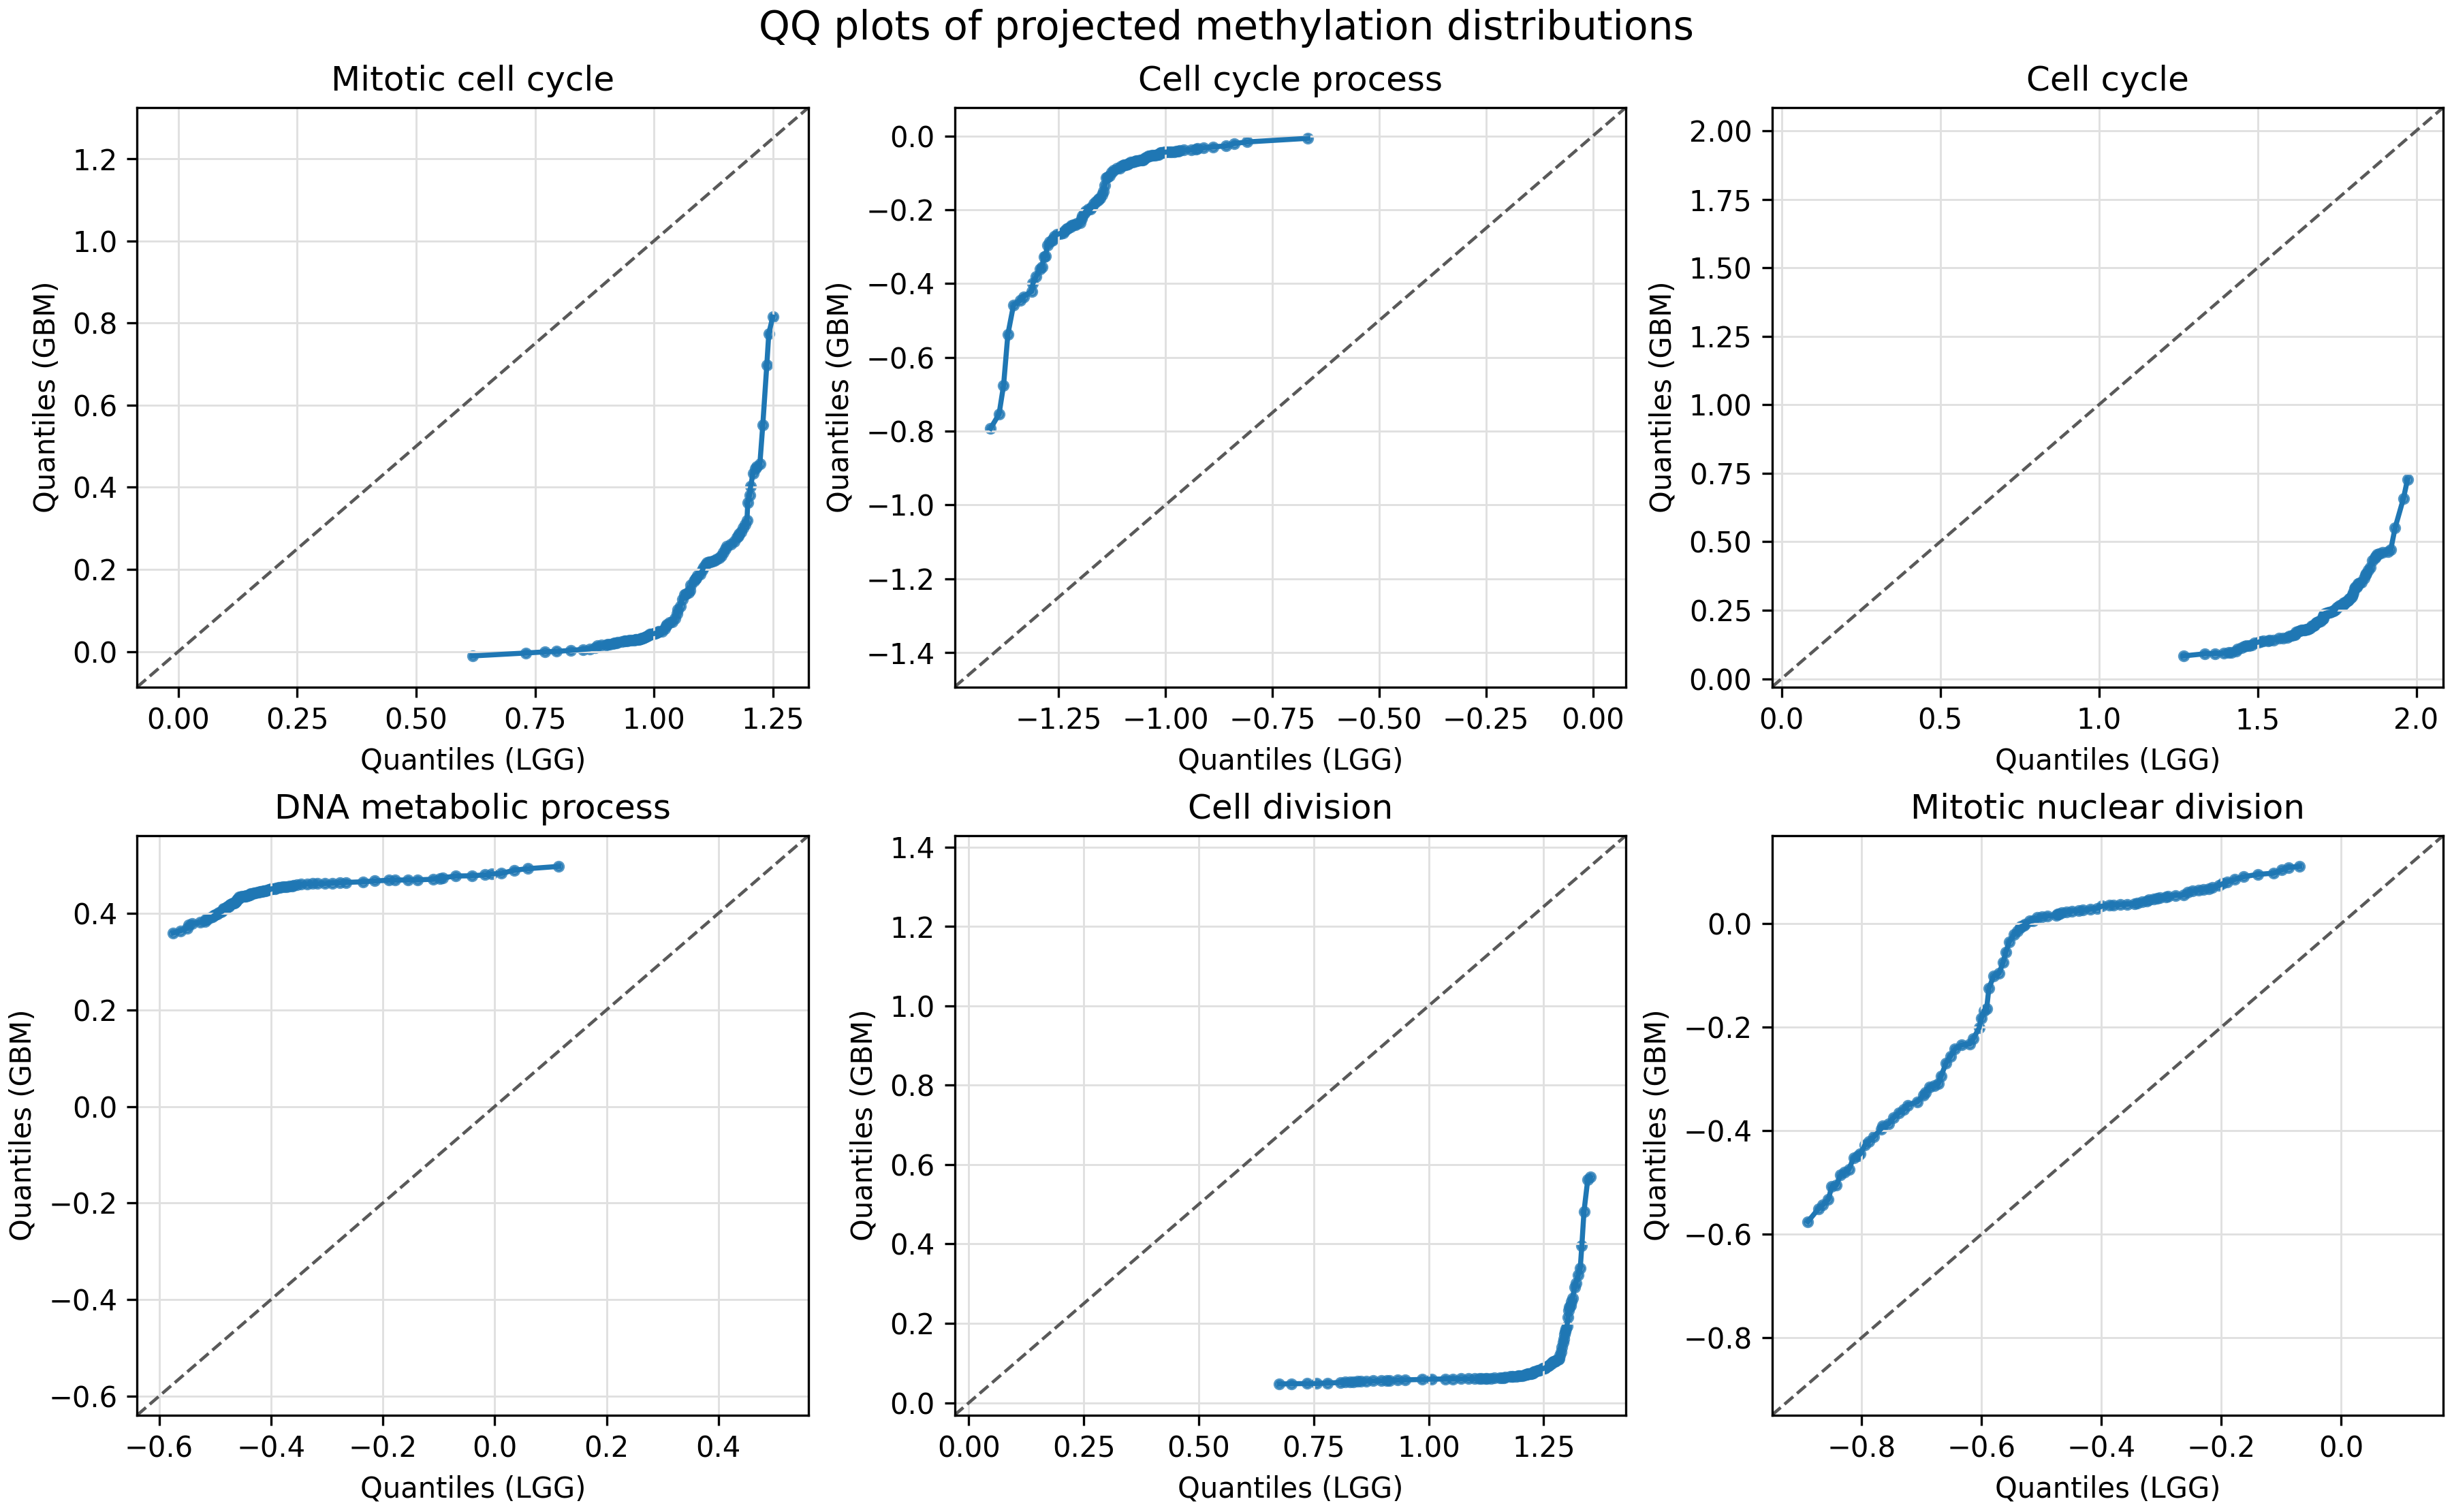
\includegraphics[width=0.82\linewidth,height=0.74\textheight,keepaspectratio]{fig3.png}
\end{center}
\end{frame}

\begin{frame}{整体结论}
\small
\begin{itemize}
  \item 实验一：MSWD 在 Model A 稀疏衰减均值差异下具备最强 power。
  \item 实验二：bootstrap 阈值解释了 Proposed 方法如何做拒绝判定。
  \item 实验三：真实 GBM 数据中，全局分布、边际基因和 GO term 层面都显著。
  \item 方法优势：max-sliced 方向搜索减少信号稀释；SCI 机制把检验和定位统一起来。
\end{itemize}
\end{frame}

\end{document}
